\documentclass[conference]{IEEEtran}
%\usepackage{a4wide}
\usepackage{NotationStyle}
\usepackage[ruled,noend,noline,slide]{algorithm2e}
\usepackage{multicol, multirow}
%\usepackage[noend]{algorithmic}
\usepackage[english]{babel}
\usepackage{amsmath,amssymb,mathrsfs,mathtext}
\usepackage{subfig}
\usepackage{graphics,graphicx,epsfig}
\usepackage{epstopdf}
\usepackage{fancybox,fancyhdr}
\usepackage{enumerate}
\usepackage{array}
\usepackage{color, soul}
%\usepackage{longtable} % longtable doesn't work with two columns
\usepackage{supertabular}
\usepackage[normalem]{ulem}
\usepackage{arydshln}
%\usepackage{accents} % for the sake of doublehat!
%\newlength{\dhatheight}
%\newcommand{\doublehat}[1]{%
%    \settoheight{\dhatheight}{\ensuremath{\hat{#1}}}%
%    \addtolength{\dhatheight}{-0.35ex}%
%    \hat{\vphantom{\rule{1pt}{\dhatheight}}%
%    \smash{\hat{#1}}}}


%\makeatletter
%\let\oldlt\longtable
%\let\endoldlt\endlongtable
%\def\longtable{\@ifnextchar[\longtable@i \longtable@ii}
%\def\longtable@i[#1]{\begin{figure}[t]
%\onecolumn
%\begin{minipage}{0.5\textwidth}
%\oldlt[#1]
%}
%\def\longtable@ii{\begin{figure}[t]
%\onecolumn
%\begin{minipage}{0.5\textwidth}
%\oldlt
%}
%\def\endlongtable{\endoldlt
%\end{minipage}
%\twocolumn
%\end{figure}}
%\makeatother

\setlength\dashlinedash{0.2pt}
\setlength\dashlinegap{4.5pt}


\newcommand{\argmax}{\mathop{\rm arg\,max}\limits}
\graphicspath{ {../code/fig/} {fig/} {../code/}}

\renewcommand{\baselinestretch}{1.3}
\begin{document}
\title{Feature generation for multiscale time series forecasting}



%Radoslav Neychev, Eric Gaussier and Vadim Strijov}
\date{Technical report (pre-draft)}
\maketitle

\begin{abstract}
The paper presents a framework for the massive multiscale time series forecast. We propose a method of constructing efficient feature description for the corresponding regression problem. The method involves feature generation and dimensionality reduction procedures. Generated features include historical information about the target time series as well as other available time series, local transformations and  multiscale features. We apply several forecasting algorithms to the resulting regression problem and investigate the quality of the forecasts for various horizon values.
\end{abstract}



\section{Introduction}
We focus on the problem of forecasting behavior of a device within the concept of Internet of Things. The device at question is monitored by a set of sensors, which produces large amount of multi-scale time series during its lifespan. These time series have various time scales since distinct sensors produce observations with various frequencies from milliseconds to weeks.  The main goal is to predict the observations of a device in a given time range.

We assume that the sampling rate of each time series is fixed and each time series has its own forecast horizon. The problem of multi-scale analysis arises in such applications as weather prediction, medical diagnosis and monitoring various sensor time series~\cite{Costa2008, Ahmed2012, Cortez2012, Ferreira2006}. Motivation for multi-scale analysis comes from the assumption that the behaviour of complex signals may be governed by  essentially different processes at various time scales. Thus, the time series should be modeled separately at each scale. This approach is used in time series classification, prediction and fault detection~\cite{Cui2016, Cortez2012, Aldrich2013}. Regardless of the goal of multi-scale analysis, it includes sequential averaging of the time series to obtain more coarse-scaled time series~\cite{Wu2013}, or, more rarely, differencing the time series for a more detailed, fine-scaled version of the time series~\cite{Jiang2011}. Averaging and differencing, which is equivalent to application of Haar's wavelet transform~\cite{Jiang2011}, may be replaced by any other pair of low and high pass wavelet filters~\cite{Chen2004} or convolution operation with some kernel function~\cite{Vespier2012}. Using multi-scale approach in time series prediction usually involves determining optimal scales~\cite{Vespier2012, Ahmed2012}, decomposition of time series into separately forecasted components and combination of the obtained forecasts.


\section{Related work}
 Along with generic methods of time series forecasting, such as Autoregressive Moving Average Models (ARMA), Autoregressive Integrated Moving Average Models (ARIMA), authors report high predictive performance of the methods, originally developed for classification or regression, applied to forecast time series~\cite{Yu2016, Kane2014, Trafalis2000, Navarrete2015, Busseti2012, Taylor2009}.  Here the input variables are the delayed observations  of the time series, and the output is the forecasted value of time series. However, the authors of~\cite{Navarrete2015} show that this prediction framework suffers from systematic error that does not converge to zero as the sample size increases, and  ensure error convergence applying cubic spline approximation to noisy data, which yields much lower RMSE in case of noisy data.

 To extend this one-step-ahead forecasting scheme to the case of multiple predictions, one may use iterative, direct or multiple output strategies~\cite{Bao2014}. Within the iterative strategy, one-step-ahead forecasts are computed recursively, with the newly predicted values of the time series used as the actual future records. A less prone to error accumulation, though more time consuming method is the direct strategy, which involves estimation of $h$ models to predict $h$ future values of the time series~\cite{Zhang2013}. Finally, the multiple input multiple output (MIMO) strategy allows to obtain $h$ prediction with at one step.  The paper~\cite{Bao2014} compares different strategies of multi-step-ahead prediction in SVR-based forecasting: direct, iterative and multiple output. Regardless of the horizon values, direct and MIMO strategies consistently achieve more accurate forecasts, than the iterative strategy, with MIMO being most accurate in most cases.


To demonstrate the application of the proposed framework of time series forecasting, we utilize Multivariate Linear Regression (MLR) as the naive approach, as well as three more complex models: Random Forests (RF)~\cite{Yu2016, Kane2014}, Support Vector Regression (SVR)~\cite{Trafalis2000, Navarrete2015, Hao2006} and artificial neural networks (ANN)~\cite{Busseti2012, Taylor2009}.  Random Forests combine decision trees with randomly generated nodes to increase the accuracy of classification or regression~\cite{Criminisi2011}. In case of regression trees, each node of the tree splits the input space into two subspaces and each leaf specifies a distinct regression model, which is used for prediction if the input is found in the corresponding region of the input space. Predictions of the trees in the forest are averaged, or, for the probabilistic random forest, the probabilities of the outputs are averaged. The advantage of random forests is their efficiency in case of highly dimensional data due to the randomness incorporated into selecting informative features. Since random forests are essentially ensembles of weak learners, they enjoy high generalization ability, associated with boosting algorithms.
 Similarly, the formulation of optimization problem within support vector regression promotes its robustness in case of highly dimensional data. The authors of~\cite{Trafalis2000, Hao2006} reported high predictive performance of SVR applied to time series forecasting. In case of SVR, MIMO strategy is based on multivariate SVR~\cite{PerezCruz2002}. Finally, artificial neural networks attract researches and practitioners from various domains~\cite{Taylor2009, Qiu2014}. One of the reasons for that is the ability os ANNs to model complex relationships between the input data in such fashion that does not require direct feature engineering. For more suggestions on how to combine these forecasting methods~\cite{Qiu2014, Grover2015} or use them in the multi-scale fashion we refer the reader to~\cite{Chen2004, Zhu2012, Cui2016, Bai2015, Ferrari2012}.


\section{Problem statement}
Consider a large set of time series~$\fD=\{\bs^{(q)}| \; q = 1,\dots, {Q}\}$, where each real-valued time series~$\bs$
\[ \bs = [s_1, \dots, s_i, \dots, s_{T}], ~~ s_i = s(t_i),\quad 0 \leq t_i \leq t_{\max}\]
is a sequence of observations $s_i = s(t_i)$ of some real-valued signal $s(t)$.
Each time series $\bs^{(q)}$ has its own sampling rate $1/\tau^{(q)}$:
\[t_i^{(q)} = {i}\cdot\tau^{(q)}.\]

 The task is to obtain forecasts $\hat{s}(t_i)$ of $\bs \in \fD$ for  $\dtr <  t_i \leq T_{\max} + \dtr$, given the set  $\fD$ (see Fig.~\ref{fg:online_frc}, \ref{fg:retrospective}). The forecasts $\hat{\bs}$ should minimise symmetric mean absolute percentage error:
 \begin{equation}\label{eq:MAPE}
 SMAPE(\bs, \hat{\bs}) = \frac{1}{r}\sum_{i = 1}^{r} \frac{2|s_i - \hat{s}_i|}{|s_i + \hat{s}_i|}. \end{equation}
 Here and throughout this paper we assume that each time series are standardized. 
 

%Here MAPE is evaluated for the retrospective forecasts~\ref{fg:retrospective}, where the most recent historical samples $\bx_0^{*}$ are concealed and forecasted as if they were unknown. Then the quality of the model $\fx$ is evaluated according to its performance on these concealed samples.

\begin{figure}[!ht]
\centering
\subfloat[]{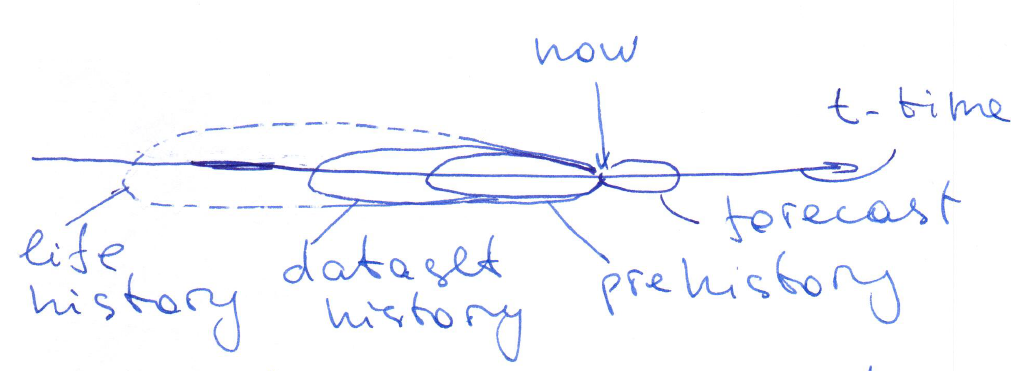
\includegraphics[width=0.4\textwidth]{online_forecasting_paradigm.png}
\label{fg:online_frc}} \\
\centering \subfloat[]{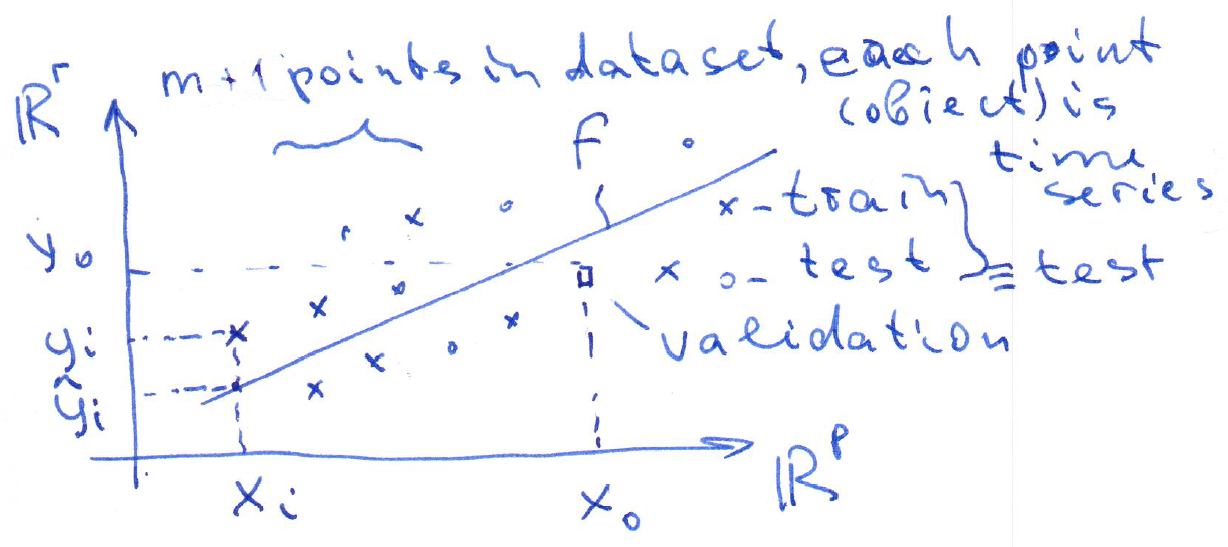
\includegraphics[width=0.4\textwidth]{forecasting_model.png}
%\input{fig/forecasting_model.eps_tex}
\label{fg:forecasting}
}
\caption{Forecasting (a) as regression problem (b).}
\end{figure}




\subsection{Design matrix}

\begin{figure}[!ht]
\centering
\subfloat[]{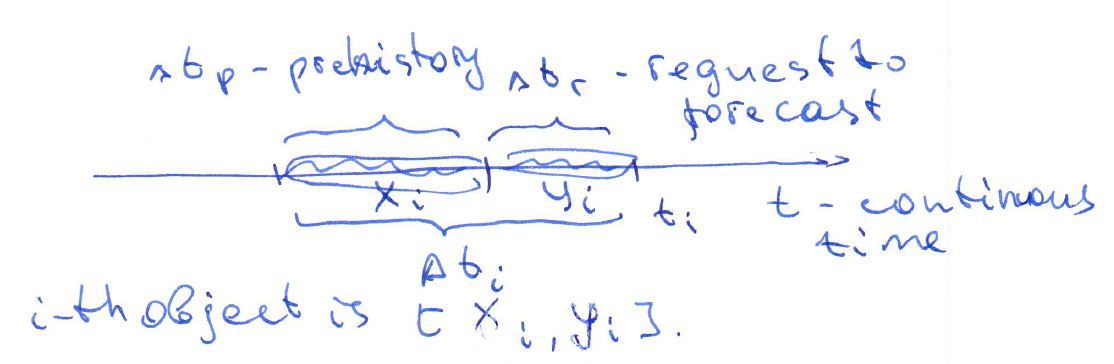
\includegraphics[width=0.4\textwidth]{draw_object.png}\label{fg:draw}} \\
\centering\subfloat[]{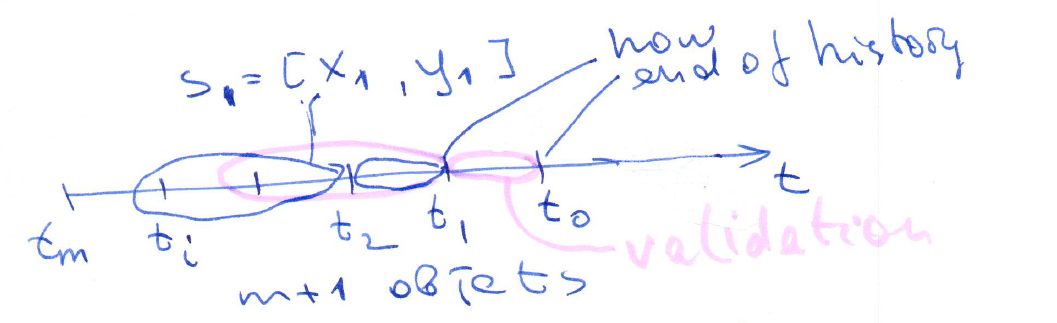
\includegraphics[width=0.4\textwidth]{design_matrix_generation.png}\label{fg:design}}
\caption{Draw an object from time series history.}
\end{figure}
 We consider the forecasting problem as the multivariate regression problem, where target variables are the vectors of lagged values $s(t_i)$ of all the time series $\bs \in \fD$.
 
Let $\bx^{*}$ denote rows of the design matrix~$\bX^*$ for the regression problem. Each vector~$\bx^{*} = [\bx| \by]$ collects all the time series over the time period~$\dtp$ (Fig.~\ref{fg:draw}), which stands for the local \emph{prehistory}. The vector $\bx^{*}$ includes samples from previous history of time series from $\fD$ as well as any derivatives or \emph{generated features}. We describe the types of generated features in Section~\ref{sc:feature_generation}.

The design matrix~$\bX^*$ for the multiscale autoregressive problem statement is constructed  as follows (Fig.~\ref{fg:design}). Let $\bs^{(q)}_i$ denote the~$i$-th segment of the time series $\bs^{(q)}$
\begin{equation}\label{eq:segment}
[\bx^{(q)}_i | \by^{(q)}_i] = \end{equation}
\[ \underbrace{s^{(q)}(t_i-\dtr-\dtp),\dots,}_{\bx^{(q)}_i} \underbrace{s^{(q)}(t_i-\dtr),\dots,s^{(q)}(t_i))}_{\by^{(q)}_i}], \]

where~$s^{(q)}(t)$ is an element of time series~$\bs^{(q)}$. To construct the design matrix, select $t_i$, $i = 1, \dots, m$ from $\Gs = \{t_1, \dots, t_T\}$ such that segments $\bs_i = [\x_i|\y_i]$ cover time series $\bs$
%\begin{equation}\label{eq:strategy2} \{s(t_{1}), \dots, s(t_{\max})\} = \bigcup_{i=1}^{q-1} \{s(t_i-\Delta t_\text{r}),\dots,s(t_i)\}\end{equation}
without intersection in target parts  $\y_i$:
\begin{equation}\label{eq:strategy2} |t_{i+1} - t_i| > \dtr.
\end{equation}
Following~\eqref{eq:segment} and~\eqref{eq:strategy2}, extract segments $[\bx^{(q)}_i | \by^{(q)}_i]$, $i = 1, \dots, m$ from all time series $\bs^{(q)} \in \fD$ and form the matrix
 \begin{equation}\label{eq:design_matrix}
\bX^*= \left[
\begin{array}{c|c}
\underset{1{\times}n}{\x} & \underset{1{\times}r}{{\by}}  \\
\hline
 \underset{m{\times}n}\bX & \underset{m{\times}r}\bY  \\
 %\hline
 \end{array}
\right] = \end{equation}
\[ \left[
\begin{array}{lll|lll}
%\bx^{(1)} & \dots & \bx^{(Q)} & \by^{(1)} &  \dots & {\by}^{(Q)}   \\
%\hline
\bx_m^{(1)}  & \dots & \bx_m^{(Q)} & \by_m^{(1)} &  \dots & \by_m^{(Q)}   \\
\vdots & \vdots & \ddots & \vdots & \vdots & \ddots  \\
\bx_1^{(1)} & \dots & \bx_1^{(Q)} & \by_1^{(1)}  & \dots & \by_1^{(Q)}   \\


\end{array}
\right]. \]

Denote a row from the pair~$\bY,\bX$ as $\by,\bx$ and call these vectors the target and the features.

\begin{figure}[!ht]
\centering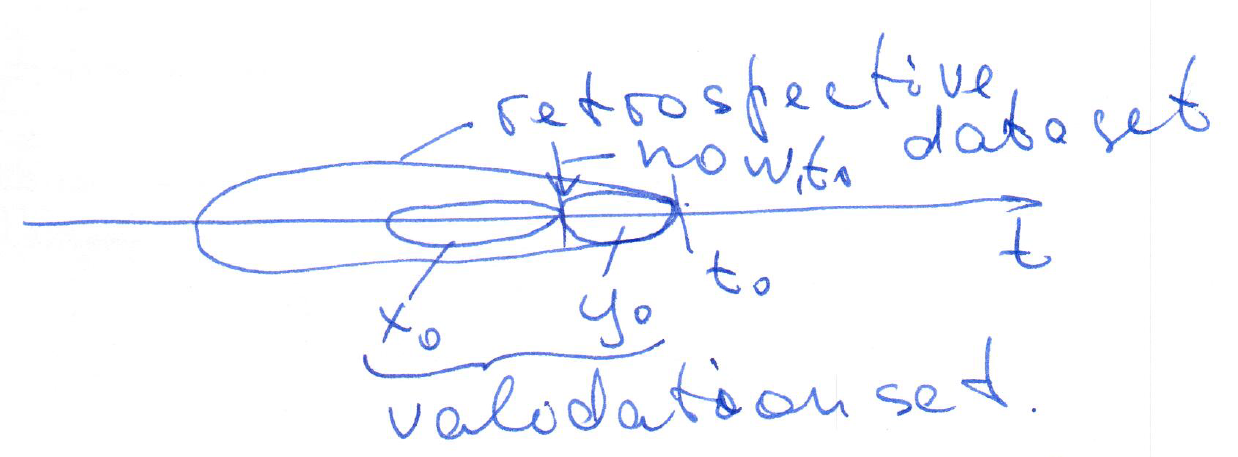
\includegraphics[width=0.4\textwidth]{retrospective_validation.png}
\caption{\hl{Retrospective forecast includes most recent samples in data set.}\label{fg:retrospective}}
\end{figure}

Now we are able the regression problem as follows:
\begin{equation}\label{eq:regression_problem}
\hat{\y} = f(\x, \hat{\w}), ~\hat{\w} = \argmin_{\hat{\w}}S\bigl(\bw|\fx(\bw,\bx),\by\bigr). %\text{~where~}
\end{equation}
Here the error function is given by $SMAPE$~\eqref{eq:MAPE} for each segment $[\x_i \by_i]$, averaged over all segments $i = 1, \dots, m$ in the test set:
\[ S\bigl(\bw|\fx(\bw,\bx),\by\bigr) = \frac{r}{m}\sum_{i=1}^{m} SMAPE(\y_i, f(\x_i, \w)).\]

\section{Feature generation}\label{sc:feature_generation}
Denote the generated feature vector as~$\vf$. This vector consists of concatenated row-vectors~$\vf=[\vf^{(1)},\dots,\vf^{(Q)}]$, which corresponds to time series local histories ~$\bs=[\bs^{(1)},\dots,\bs^{(Q)}]$, modified with set of transformations~$G$. The elements~$g:\bs\to\vf$ of this set are listed below. The augmented feature set $\vf$ includes
\begin{enumerate}[1)]
\item the local history of all time series themselves,
\item transformations (non-parametric and parametric) of local history,
\item parameters of the local models,
\item distances to the centroids of local clusters.
\end{enumerate}



\subsection{Transformations of local history}
We use non-parametric and parametric functions to generate features. The purpose of this block of features is to introduce nonlinearities into the feature space of regression problem~\eqref{eq:regression_problem}.

The parametric procedure involves two optimization problems. The first one fixes the vector~$\hat\bb$, collected over all the primitive functions~$g=g(\bb,s) \in G$, which generate features~$\vf$:
\[
\hat\bw = \arg\min_{\bw} S\bigl(\bw|\fx(\bw,\vf),\by\bigr),\quad
\text{where}
\quad \vf = g(\hat\bb,\bs).
\]
The second one optimizes the transformation parameters~$\hat\bb$ given the obtained model parameters~$\bw$
\[
\hat\bb = \arg\min_{\bb} S\bigl(\bb|\fx(\hat\bw,\vf),\by\bigr).
\]
This parametric feature generation procedure repeats these problems until vectors~$\hat\bw,\hat\bb$ converge. The initial values of the parameters~$\bb$ are assigned empirically.

\subsection{Convolutions, statistics and parameters of local history}
These block of feature generation functions includes convolutions, time averaging and differencing, and basic statistics of each time series, such as mean and standard deviation, minimum and maximum of the input $\bx$. The features from these part can be seen as applying Haar's wavelet transform to each segment~\cite{Jiang2011}. Motivation for this comes from assuming the multi-scale nature of the time series: complex signals may be governed by essentially different processes at various time scales. Averaging of the time series allows to obtain more coarse-scaled time series, while differencing the time series provides a more detailed, fine-scaled version of the time series.


\subsection{Parameters of local history forecast}
For the time series~$\bs$ construct the Hankel matrix with a~period~$k$ and shift~$p$, so~that for~$\bs = [s_1,\dots,s_T]$ the matrix
\[
\bH^* =
\left[ \begin{array}{c|cc}
s_T  & \dots & s_{T-k+1} \\
\vdots & \ddots & \vdots \\
s_{k+p} & \dots & s_{1+p}\\
s_k & \dots & s_1 \\
\end{array}
\right],
\text{~where~} 1\geqslant p \geqslant k .
\]
Reconstruct the regression to the first column of the matrix~$\bH^*=[\bh, \bH]$ and denote its least square parameters as the feature vector
\[
\boldsymbol{\phi}^{(q)} = \arg\min \| \bh-\bH \boldsymbol{\phi}\|_2^2.
\]
For the time series~$\bs^{(q)}$, $q=1,\dots, Q$ use the parameters $\boldsymbol{\phi}^{(q)}$ as the features.

\subsection{Distances to centroids of local clusters}
This procedure applies the kernel trick to the time series. For given local history time series~$\bx_i^{(q)}$, $q=1,\dots, Q$ compute $k$-means centroids~$\bc_p^{(q)}$, $p = 1, \dots, P$.  With the selected $k$-means distance function~$\rho$ construct the feature vector
\[
\vf_i^{(q)} = [\rho(\bc_1^{(q)},\bs_i^{(q)}),\dots,\rho(\bc^{(q)}_P,\bs_i^{(q)})] \in \R_+^P.
\]
This $k$-means of another clustering procedure may use internal parameters, so that there are no parameters to be included to the feature vector or to the forecasting model.

\begin{algorithm}[!h]
%\DontPrintSemicolon
\KwData{Object-feature matrix $\bX^{*} \in \mathbb{R}^{m\times(n+r)}$. Train to test ratio $\alpha \in [0, 1]$.}
 \KwResult{Train and test, $\bX^{*}_{\text{train}}$, $\bX^{*}_{\text{test}}$.}
 Set train set and test set sizes:

 $ \quad m_{\text{train}} = \lfloor\alpha\cdot m\rfloor, \quad m_{\text{test}} = m - m_{\text{train}} $ \; %(1-\alpha)(m-1)
 Decompose matrix $\bX^{*}$ into train and test matrices $\bX^{*}_{\text{train}}$, $\bX^{*}_{\text{test}}$:
 \[\bX^{*} = \left[\begin{array}{c|c}
 \underset{m_{\text{test}}{\times}n}{\bX_{\text{test}}} & \underset{m_{\text{test}}{\times}r}{\bY_{\text{test}}}  \\
 \hdashline
 \underset{m_{\text{train}}{\times}n}{\bX_{\text{train}}}  & \underset{m_{\text{train}}{\times}r}{\bY_{\text{train}}}
 \end{array}\right]
 \]
  \caption{Initial train-test splitting procedure.}\label{alg:train_test}
\end{algorithm}

\section{Testing procedure}
The algorithm below describes the procedure used to evaluate the forecasting errors within the proposed framework given the model $\fx$,  data matrix $\bX^{*} \in \mathbb{R}^{m\times(n+r)}$ and fixed parameters train to test ratio $\alpha$, minimal sample (test) size $m_{\min}$. This procedure involves creation of design matrix~\eqref{eq:design_matrix}, generation of augmented feature description $\vf$ and, since it is likely to be redundant, dimensionality reduction. Here we use principal component analysis (PCA) and nonlinear PCA~\cite{}.
\begin{enumerate}[1)]
\item Create design matrix $\bX^{*}$ according to~\eqref{eq:design_matrix} from $\fD$.  
\item Split matrix $\bX^{*}$ into train and test matrices $\bX^{*}_{\text{train}}$ and $\bX^{*}_{\text{test}}$ 
according to the train-test splitting procedure~\ref{alg:train_test}\;
\item Augment $\bX^{*}_{\text{train}}$ with generated features $\vf$\;
\item Reduce dimensionality of $\bX^{*}_{\text{train}}$ \;
\item Optimize hyper parameters of the model $\fx$, using $\bX^{*}_{\text{train}}$\;
\item
For $k$ in $\{1, \dots,  m_{\text{test}} - m_{\min}\}$ repeat:
\begin{itemize}
\item define $\bX^{*}_{\text{train}, i}$ as $(i+1)$-th to $(i+ m_{\min} + 1)$-th rows of $\bX^{*}_{\text{test}}$ and
  $\bx^{*}_{\text{val}, i}$ as the $i$-th row of $\bX^{*}_{\text{test}}$\;

 \[\bX^{*}_{\text{test}} = \left[\begin{array}{c|c}
 \dots & \dots \\
 \hline
 \underset{1{\times}n}{\bx_{\text{val}, i}} & \underset{1{\times}r}{\by_{\text{val}, i}}  \\
 \hdashline
 \underset{m_{\min}{\times}n}{\bX_{\text{train}, i}}  & \underset{m_{\min}{\times}r}{\bY_{\text{train}, i}} \\
 \hline
 \dots & \dots \\
 \end{array}\right]
 \]
\item apply feature transformation to $\bX^{*}_{\text{train}, i}$, $\bX^{*}_{\text{val}, i}$\;
\item  train forecasting model $\fx(\x, \hat{\w}_i)$, using $\bX^{*}_{\text{train}, i}$\;
\item  obtain vector of residuals $\veps  = \by_{\text{val}, i} - \fx(\bx_{\text{val}, i}, \hat{\w}_i)$\;
\item  compute forecasting quality:
  \[ {SMAPE}(i)  = \frac{1}{r} \sum_{t=1}^{r} \frac{2|\varepsilon_{t}|}{|2(y_{\text{val}, i})_t - \varepsilon_{t}|};\]
\end{itemize}
\item
  Return $SMAPE$, averaged over data splits:
  \[ \text{Error}  = \frac{1}{m_{\text{test}} - m_{\min}} \sum_{i=1}^{m_{\text{test}} - m_{\min}} {SMAPE}(i).\]
\end{enumerate}
The models that we use are listed in the table~\ref{tb:regr_mdl} along with the optimized hyper parameters.


\section{Computational experiment}
The goal of the experiment is to study the performance of multivariate regression approach to the problem of
time series forecasting.

This section presents the results of computational comparison of the forecasting models presented above. To test each model, we used several datasets, described below.
\begin{table}\caption{Regression models.}\label{tb:regr_mdl}
\begin{tabular}{|p{4cm}|p{4cm}|}
\hline
Model name & Hyper parameters \\
\hline
 multivariate linear regression (MVR) with $l_2$-regularization & regularization coefficient \\
 \hline
%\[f(\bx, \bW) = \bx\bW , ~~ \hat{\bW} = \argmin_{\bW} S(\bW) + \lambda||\bW||_2^2, \]
support vector regression (SVR) & parameters $C$, $\lambda$, $\varepsilon$ \\
%where the regression function also has the linear form $f(\bX, \{\bW, \bb\}) = \bx\bW + \bb$, but the optimization problem is more complex:
%    \[ \hat{\bW} = \argmin_{\bW,\;\vx,\;\vx^{*}} \frac{1}{2}||\bW||_2^2 + C
%    \sum_{i, j}(\xi_{ij} + \xi_{ij}^{*}), \text{~subject to~}\]
%    \[ \begin{cases} -\veps - \vx^{*}_i \leq \by_i - \bx_i\bW  - \bb \leq \veps + \vx_i, \\
%     \xi_{ij}\xi^{*}_{ij} > 0.
%    \end{cases}\]
\hline 
artificial neural network (ANN) &  number of hidden layers, hidden layers size \\
\hline random forest (RF) & number of trees, number of variables per tree\\
\hline
\end{tabular}
\end{table}
\subsection{Datasets}
\begin{itemize}
\item Energy-Weather dataset. The dataset consists of the Polish electricity load time series~\cite{EnergyWeatherData} and weather time series in Warsaw (Longtitude: 21.25, Latitude: 52.30, Elevation: 94). Energy time series contain hourly records (total of 52512 observations), while weather time series were measured daily and contain 2188 observations. The multiscale time series correspond to the period of 1999 to 2004.
    
\item  The Energy-Weather dataset was used to generate several artificial datasets. 

\item Accelerometry dataset. This dataset consists of accelerometry time series from the Human Activity Sensing Consortium~\cite{HASCdata}. Each time series in the datasets is a sequence of acceleration records. The time series were recorded for 120 seconds while a subject performed a sequence of activities: stay, walk, jog, skip, stair up or stair down. The sampling rate varies between 10 and 100Hz, but stays constant for each time series.
\item Financial dataset~\cite{NNcompetition}.  The dataset A (final, complete) from the 2006/07 Forecasting Competition for Neural Networks \& Computational Intelligence. The dataset contains 111 monthly time series drawn from homogeneous population of empirical business time series.
\end{itemize}

\subsection{Experimental results}
Each time series from the datasets was converted to the design matrix~\eqref{eq:design_matrix} and used as input data to train regression models according to~\eqref{eq:regression_problem}.

Table~\ref{fg:feature_selection_res_HASC1} lists forecasting errors for the proposed feature generation strategies applied to the test time series from the HASC dataset.

Fig.~\ref{fg:target_data} displays an example of target time series HASC1001 and the results of forecasting a single segment of this time series with the baseline models.

Fig.~\ref{fg:feature_gen_frc} illustrates the results of regression built on the design matrix, augmented with the particular data generation method.

Fig.~\ref{fg:pca_frc} demonstrates the forecasts, obtained by each model in the proposed framework. Here the design matrix was augmented with the generated features and PCA was applied to select a subset of features.



\begin{table}
\begin{tabular}{|c|c|c|c|c|}
\hline
Feature set & Models &MAPE test & MAPE train & AIC\\
\hline
\multirow{4}{*}{History} &VAR &   7.215 &    0.067 &    1427.927\\
\cline{2-5}
 &SVR &   0.718 &    0.320 &    1396.463\\
\cline{2-5}
 &Random Forest &   0.463 &    0.206 &    1388.668\\
\cline{2-5}
 &Neural network &   0.624 &    0.407 &    1389.319\\
\cline{2-5}
\hline
\multirow{4}{*}{SSA} &VAR &   0.755 &    0.402 &    1375.959\\
\cline{2-5}
 &SVR &   1.348 &    0.434 &    1401.053\\
\cline{2-5}
 &Random Forest &   0.746 &    0.335 &    1413.181\\
\cline{2-5}
 &Neural network &   0.544 &    0.387 &    1379.299\\
\cline{2-5}
\hline
\multirow{4}{*}{Cubic} &VAR &   0.562 &    0.382 &    1371.387\\
\cline{2-5}
 &SVR &   0.779 &    0.418 &    1373.299\\
\cline{2-5}
 &Random Forest &   0.647 &    0.320 &    1412.390\\
\cline{2-5}
 &Neural network &   0.795 &    0.387 &    1371.354\\
\cline{2-5}
\hline
\multirow{4}{*}{Conv} &VAR &   2.182 &    2.180 &    2252.866\\
\cline{2-5}
 &SVR &   2.986 &    0.537 &    1413.103\\
\cline{2-5}
 &Random Forest &   0.583 &    0.323 &    1408.932\\
\cline{2-5}
 &Neural network &   0.743 &    0.406 &    1373.955\\
\cline{2-5}
\hline
\multirow{4}{*}{NW} &VAR &   2.021 &    0.041 &    1605.095\\
\cline{2-5}
 &SVR &   0.714 &    0.323 &    1398.156\\
\cline{2-5}
 &Random Forest &   0.427 &    0.195 &    1381.996\\
\cline{2-5}
 &Neural network &   0.815 &    0.425 &    1389.418\\
\cline{2-5}
\hline
\multirow{4}{*}{All} &VAR &   2.000 &    2.000 &    9910.259\\
\cline{2-5}
 &SVR &   0.751 &    0.324 &    1395.951\\
\cline{2-5}
 &Random Forest &   0.415 &    0.194 &    1381.906\\
\cline{2-5}
 &Neural network &   1.254 &    0.399 &    1381.405\\
\cline{2-5}
\hline
\multirow{4}{*}{PCA} &VAR &   0.712 &    0.310 &    1388.756\\
\cline{2-5}
 &SVR &   0.748 &    0.323 &    1395.828\\
\cline{2-5}
 &Random Forest &   0.504 &    0.214 &    1378.500\\
\cline{2-5}
 &Neural network &   0.563 &    0.392 &    1377.608\\
\cline{2-5}
\hline
\end{tabular}
\caption{Forecasting errors measured as symmetric MAPE.}
\label{fg:feature_selection_res_HASC1}
\end{table}


\begin{figure}
\centering
%\subfloat[]{\includegraphics[width=0.18\textwidth]{fig/feature_selection/HascData/data_HASC1001.png}}
\subfloat[]{\includegraphics[trim= 2cm 0 0 15cm,clip,width=0.25\textwidth]{fig/feature_selection/HascData/data_segms_HASC1001.png}}
\subfloat[]{\includegraphics[trim= 2cm 0 0 15cm,clip,width=0.25\textwidth]{fig/feature_selection/HascData/res_HASC1001.png}}
\caption{Accelerometry time series from HASC project.
(a) Target segments of the time series HASC1001. (b) Forecasting results for	HASC1001 (VAR, SVR, Random Forest, Neural network).}\label{fg:target_data}
\end{figure}


\begin{figure}
\centering
\subfloat[VAR]{\includegraphics[trim= 2cm 0 0 15cm,clip, width=0.25\textwidth]{fig/frc_analysis/HascData/stats_HASC1001VAR.png}}
\subfloat[VAR]{\includegraphics[trim= 2cm 0 0 15cm,clip, width=0.25\textwidth]{fig/frc_analysis/HascData/stats_HASC1001_fs_VAR.png}} \\
\subfloat[SVR]{\includegraphics[trim= 2cm 0 0 15cm,clip,width=0.25\textwidth]{fig/frc_analysis/HascData/stats_HASC1001SVR.png}}
\subfloat[SVR]{\includegraphics[trim= 2cm 0 0 15cm,clip,width=0.25\textwidth]{fig/frc_analysis/HascData/stats_HASC1001_fs_SVR.png}}\\
\subfloat[Random forest]{\includegraphics[trim= 2cm 0 0 15cm,clip, width=0.25\textwidth]{fig/frc_analysis/HascData/stats_HASC1001Random_Forest.png}}
\subfloat[Random forest]{\includegraphics[trim= 2cm 0 0 15cm,clip, width=0.25\textwidth]{fig/frc_analysis/HascData/stats_HASC1001_fs_Random_Forest.png}} \\
\subfloat[ANN]{\includegraphics[trim= 2cm 0 0 15cm,clip, width=0.25\textwidth]{fig/frc_analysis/HascData/stats_HASC1001Neural_network.png}}
\subfloat[ANN]{\includegraphics[trim= 2cm 0 0 15cm,clip, width=0.25\textwidth]{fig/frc_analysis/HascData/stats_HASC1001_fs_Neural_network.png}}\\
\caption{Mean residual by number of forecasted point for historical data only and all generation strategies with PCA.}
\end{figure}


\begin{figure}
\centering
\subfloat[SSA]{\includegraphics[trim= 2cm 0 0 15cm,clip, width=0.25\textwidth]{fig/feature_selection/HascData/res_HASC1001_fs_SSA.png}}
\subfloat[Cubic]{\includegraphics[trim= 2cm 0 0 15cm,clip, width=0.25\textwidth]{fig/feature_selection/HascData/res_HASC1001_fs_Cubic.png}} \\
\subfloat[Conv]{\includegraphics[trim= 2cm 0 0 15cm,clip, width=0.25\textwidth]{fig/feature_selection/HascData/res_HASC1001_fs_Conv.png}}
\subfloat[NW]{\includegraphics[trim= 2cm 0 0 15cm,clip, width=0.25\textwidth]{fig/feature_selection/HascData/res_HASC1001_fs_NW.png}} \\
\subfloat[All]{\includegraphics[trim= 2cm 0 0 15cm,clip, width=0.25\textwidth]{fig/feature_selection/HascData/res_HASC1001_fs_all.png}}
\subfloat[PCA]{\includegraphics[trim= 2cm 0 0 15cm,clip, width=0.25\textwidth]{fig/feature_selection/HascData/res_HASC1001_fs_pca.png}} \\
\caption{Forecasting results for various feature generation strategies, HASC1001.}\label{fg:feature_gen_frc}
\end{figure}


\begin{figure}
\centering
\subfloat[VAR]{\includegraphics[trim= 2cm 0 0 15cm,clip, width=0.25\textwidth]{fig/feature_selection/HascData/res_HASC1001_VAR_fs_pca.png}}
\subfloat[SVR]{\includegraphics[trim= 2cm 0 0 15cm,clip, width=0.25\textwidth]{fig/feature_selection/HascData/res_HASC1001_SVR_fs_pca.png}}\\
\subfloat[Random Forest]{\includegraphics[trim= 2cm 0 0 15cm,clip, width=0.25\textwidth]{fig/feature_selection/HascData/res_HASC1001_Random_Forest_fs_pca.png}}
\subfloat[ANN]{\includegraphics[trim= 2cm 0 0 15cm,clip, width=0.25\textwidth]{fig/feature_selection/HascData/res_HASC1001_Neural_network_fs_pca.png}}\\
\caption{ Forecasting results for HASC1001 with all feature generation strategies applied and PCA feature selection.}\label{fg:pca_frc}
\end{figure}

\nocite{*}
\bibliographystyle{IEEEtran}%{unsrt}
\bibliography{MultiscaleForecasting}


\end{document}
%%%%%%%%%%%%%%%%%%%%%%%%%%%%%%%%%%%%%%%%%%%%%%%%%%%%%%%%%%%%%%%%%%%%%%%%%%%%%%%%%%%%%%%%%%%%%%%%%%%%%

%\begin{algorithm}[!h]
%%\DontPrintSemicolon
%%\textbf{\emph{ComputeForecastingErrors()}}\\
% \KwData{$\bX^{*} \in \mathbb{R}^{m\times(n+r)}$. Parameters: sample size $m$, train to test ratio $\alpha$, minimal sample (test) size $m_{\min}$.}
% \KwResult{Forecasting error.}
% Decompose matrix $\bX^{*}$ into train and test matrices:
% \[\bX^{*}_{\text{train}}, \; \bX^{*}_{\text{test}} = TrainTestSplit(\bX^{*}, \alpha);\]
% Optimize hyperparameters $\hat{\beta}$ of the model $\fx$, using $\bX^{*}_{\text{train}}$ \;
% \For{$i$ in $\{1, \dots,  m_{\text{test}} - m_{\min}\}$:}{
% define $\bX^{*}_{\text{train}, i}$ as $(i+1)$-th to $(i+ m_{\min} + 1)$-th rows of $\bX^{*}_{\text{test}}$ \;
% define $\bx^{*}_{\text{val}, i}$ as the $i$-th row of $\bX^{*}_{\text{test}}$ \;
%  train forecasting model $\fx(\x, \hat{\w}_i, \hat{\beta})$, using $\bX^{*}_{\text{train}, i}$ and \;
%  obtain vector of residuals $\veps  = \by_{\text{val}, i} - \fx(\bx_{\text{val}, i}, \hat{\w}_i, \hat{\beta})$ \;
%  compute forecasting quality:
%  \[ {SMAPE}(i)  = \frac{1}{r} \sum_{t=1}^{r} \frac{2|\varepsilon_{t}|}{|2(y_{\text{val}, i})_t - \varepsilon_{t}|};\]
%  }
%  Return $SMAPE$, averaged over data splits:
%  \[ \text{Error}  = \frac{1}{m_{\text{test}} - m_{\min}} \sum_{i=1}^{m_{\text{test}} - m_{\min}} {SMAPE}(i).\]
%  \bigskip
% \caption{Compute forecasting errors imitating rolling forecast procedure.}\label{alg:train_test_rmse}
%\end{algorithm}
%
%\begin{algorithm}[!h]
%\DontPrintSemicolon
%\textbf{\emph{TrainTestSplit()}}\\
%\KwData{Object-feature matrix $\bX^{*} \in \mathbb{R}^{m\times(n+r)}$. Train to test ratio $\alpha \in [0, 1]$.}
% \KwResult{Train and test, $\bX^{*}_{\text{test}}$, $\bX^{*}_{\text{val}}$.}
% Set train set and test set sizes:
%
% $ \quad m_{\text{train}} = \lfloor\alpha\cdot m\rfloor, \quad m_{\text{test}} = m - m_{\text{train}} $ \; %(1-\alpha)(m-1)
% Decompose matrix $\bX^{*}$ into train and test matrices $\bX^{*}_{\text{train}}$, $\bX^{*}_{\text{test}}$:
% \[\bX^{*} = \left[\begin{array}{c|c}
% \underset{m_{\text{test}}{\times}n}{\bX_{\text{test}}} & \underset{m_{\text{test}}{\times}r}{\bY_{\text{test}}}  \\
% \hdashline
% \underset{m_{\text{train}}{\times}n}{\bX_{\text{train}}}  & \underset{m_{\text{train}}{\times}r}{\bY_{\text{train}}}
% \end{array}\right]
% \]
%  \caption{Initial train-test split procedure.}\label{alg:train_test_rmse}
%\end{algorithm}


%\begin{figure}
%\centering
%\subfloat[VAR]{\includegraphics[trim= 2cm 0 0 15cm,clip, width=0.25\textwidth]{fig/feature_selection/HascData/res_HASC1001_VAR.png}}
%\subfloat[SVR]{\includegraphics[trim= 2cm 0 0 15cm,clip, width=0.25\textwidth]{fig/feature_selection/HascData/res_HASC1001_SVR.png}}\\
%\subfloat[Random forest]{\includegraphics[trim= 2cm 0 0 15cm,clip, width=0.25\textwidth]{fig/feature_selection/HascData/res_HASC1001_Random_Forest.png}}
%\subfloat[ANN]{\includegraphics[trim= 2cm 0 0 15cm,clip, width=0.25\textwidth]{fig/feature_selection/HascData/res_HASC1001_Neural_network.png}}\\
%\caption{Forecasts of HASC1001 with historical features only.}\label{fg:hitorical_data_frc}
%\end{figure}



%\begin{figure}
%\centering
%\subfloat[VAR]{\includegraphics[trim= 2cm 0 0 15cm,clip, width=0.25\textwidth]{fig/feature_selection/HascData/res_HASC1001_VAR_fs_Conv.png}}
%\subfloat[SVR]{\includegraphics[trim= 2cm 0 0 15cm,clip,width=0.25\textwidth]{fig/feature_selection/HascData/res_HASC1001_SVR_fs_Conv.png}}\\
%\subfloat[Random forest]{\includegraphics[trim= 2cm 0 0 15cm,clip, width=0.25\textwidth]{fig/feature_selection/HascData/res_HASC1001_Random_Forest_fs_Conv.png}}
%\subfloat[ANN]{\includegraphics[trim= 2cm 0 0 15cm,clip, width=0.25\textwidth]{fig/feature_selection/HascData/res_HASC1001_Neural_network_fs_Conv.png}}\\
%\caption{Forecasts of HASC1001 with convolutional features added.}
%\end{figure}

%\begin{figure}
%\centering
%\subfloat[SSA]{\includegraphics[trim= 2cm 0 0 15cm,clip, width=0.25\textwidth]{fig/feature_selection/HascData/generation_HASC1001_fs_SSA.png}}
%\subfloat[SSA]{\includegraphics[trim= 2cm 0 0 15cm,clip, width=0.25\textwidth]{fig/feature_selection/HascData/res_HASC1001_fs_SSA.png}}\\
%\subfloat[Cubic]{\includegraphics[trim= 2cm 0 0 15cm,clip, width=0.25\textwidth]{fig/feature_selection/HascData/generation_HASC1001_fs_Cubic.png}}
%\subfloat[Cubic]{\includegraphics[trim= 2cm 0 0 15cm,clip, width=0.25\textwidth]{fig/feature_selection/HascData/res_HASC1001_fs_Cubic.png}} \\
%\subfloat[Conv]{\includegraphics[trim= 2cm 0 0 15cm,clip, width=0.25\textwidth]{fig/feature_selection/HascData/generation_HASC1001_fs_Conv.png}}
%\subfloat[Conv]{\includegraphics[trim= 2cm 0 0 15cm,clip, width=0.25\textwidth]{fig/feature_selection/HascData/res_HASC1001_fs_Conv.png}} \\
%\subfloat[NW]{\includegraphics[trim= 2cm 0 0 15cm,clip, width=0.25\textwidth]{fig/feature_selection/HascData/generation_HASC1001_fs_NW.png}}
%\subfloat[NW]{\includegraphics[trim= 2cm 0 0 15cm,clip, width=0.25\textwidth]{fig/feature_selection/HascData/res_HASC1001_fs_NW.png}} \\
%\subfloat[All]{\includegraphics[trim= 2cm 0 0 15cm,clip, width=0.25\textwidth]{fig/feature_selection/HascData/generation_HASC1001_fs_all.png}}
%\subfloat[All]{\includegraphics[trim= 2cm 0 0 15cm,clip, width=0.25\textwidth]{fig/feature_selection/HascData/res_HASC1001_fs_all.png}}
%\caption{Forecasting results for various feature generation strategies, HASC1001.}\label{fg:feature_gen_frc}
%\end{figure} 